\documentclass[8pt]{beamer}

\usetheme{metropolis}

\usepackage{graphicx}
\usepackage{multirow}
\usepackage{pgfplots}
\usepackage{pgfplotstable}
\usepackage{subcaption}
\usepackage{tikz}
\usepackage{transparent}

\author{Esten H{\o}yland Leonardsen}
\institute[Life Science, UiO]{UiO:Life Science, University of Oslo}
\date{12.10.22}
\title{Explainable AI in healthcare}

% TIKZ PACKAGES
\usetikzlibrary{arrows.meta}
\usetikzlibrary{calc}
\usetikzlibrary{patterns}
\usetikzlibrary{positioning}
\usetikzlibrary{shapes}

% PGFPLOTS PACKAGES
\usepgfplotslibrary{fillbetween}
\usepgfplotslibrary{groupplots}

% COLOUR
\definecolor{cb-pink}{HTML}{eeafcf}
\definecolor{cb-orange}{HTML}{e59145}
\definecolor{cb-light-brown}{HTML}{baa066}
\definecolor{cb-blue}{HTML}{3594d6}
\definecolor{cb-green}{HTML}{4dac93}
\definecolor{cb-gray}{HTML}{3a5c7d}
\definecolor{cb-light-purple}{HTML}{b45899}
\definecolor{cb-red-purple}{HTML}{c71555}
\definecolor{cb-brown}{HTML}{840000}
\definecolor{cb-blue-purple}{HTML}{662fa2}

\colorlet{cases-default}{cb-red-purple}
\colorlet{controls-default}{cb-blue}

\begin{document}

	\begin{frame}
		\maketitle
	\end{frame}

	\begin{frame}{AI in neuroimaging}
		General example of AI application in neuroimaging
	\end{frame}

	\begin{frame}{Brain age}
		\centering
		\vfill
		\fbox{
			\includegraphics[width=0.6\textwidth]{data/cole.png}
		}\\
		\vspace{0.1cm}
		"Brain age and other bodily ‘ages’: implications for neuropsychiatry."\\ Cole, James H., et al. \textit{Molecular psychiatry} (2019).
		\vfill
	\end{frame}

	\begin{frame}{Brain age}
		\centering
		\vfill
		\begin{tikzpicture}
			\node[inner sep=0pt, draw=black, label=below:] (kaufmann) at (0, 0) {
				\includegraphics[width=0.4\textwidth]{data/kaufmann.png}
			};

			\node[inner sep=0pt, draw=black] (ours) at (5, 0) {
				\includegraphics[width=0.4\textwidth]{data/ours.png}
			};

			\node[anchor=north, align=center, font=\footnotesize\linespread{0.8}\selectfont] at (kaufmann.south) {
				"Common brain disorders are associated with\\
				heritable patterns of apparent aging of the brain"\\
				Kaufmann, Tobias, et al. \textit{Nature Neuroscience} (2019)
			};
			\node[anchor=north, align=center, font=\footnotesize\linespread{0.8}\selectfont] at (ours.south)
			{
				"Deep neural networks learn general and clinically\\
				 relevant representations of the ageing brain."\\
				Leonardsen, Esten H., et al. \textit{NeuroImage} (2022)
			};

		\end{tikzpicture}
	\end{frame}

	\begin{frame}{Brain age}
		\centering
		\vfill
		\begin{tikzpicture}
			\node[inner sep=0pt, draw=black] at (0, 0) {
				\includegraphics[width=0.8\textwidth]{data/ms.png}
			};
			\node[inner sep=0pt, draw=black] at (0, 3) {
				\includegraphics[width=0.8\textwidth]{data/dementia.png}
			};
		\end{tikzpicture}
		\vfill
	\end{frame}

	\begin{frame}{Explainable AI}
		\definecolor{cb-blue}{HTML}{3594d6}
		\definecolor{cb-red-purple}{HTML}{c71555}

		\definecolor{outercolor}{RGB}{128, 128, 128}
		\newcommand{\nodesize}{11pt}
		\newcommand{\hsep}{28pt}
		\newcommand{\vsep}{14pt}

		\newcommand{\arrowwidth}{0.05cm}
		\newcommand{\innerarrow}{{Latex[length=0.1cm, width=0.15cm]}}
		\newcommand{\outerarrow}{{Latex[length=0.2cm, width=0.3cm]}}

		\def\plotwidth{11.68}
		\centering
		\vfill
		\scalebox{0.8}{
			\fbox{
				\begin{tikzpicture}
					\newcommand{\mrivsep}{0.52}
					\newcommand{\mrihsep}{0.44}

					\node[anchor=north west] at (0, 0.1) {\footnotesize{2. Apply model and LRP for individual-level predictions and relevance maps}};
					\node[anchor=north east] at (\plotwidth, 0) {};

					\newcommand{\mrilocation}[1]{($ (1, -2.2) + ####1 $)}
					\newcommand{\modellocation}[1]{($ (0.5 * \plotwidth, -2.2) + ####1 $)}
					\newcommand{\lrplocation}[1]{($ (0.5 * \plotwidth, -5.2) + ####1 $)}
					\def\maplocation{(1, -5.2)}

					\node[anchor=south, align=center, font=\scriptsize\linespread{0.85}\selectfont] at \mrilocation{(0, 0.92)} {All\\subjects};

					\newcommand{\mrialpha}{0.2}
					\colorlet{predict-fill}{cb-blue}
					\colorlet{lrp-fill}{red}

					\node[] at \mrilocation{(-1 * \mrihsep, -1.5*\mrivsep)} {
						{\transparent{\mrialpha}\includegraphics[height=0.5cm]{data/mris/slice_5.png}}
					};
					\node[] at \mrilocation{(0, -1.5*\mrivsep)} {
						{\transparent{\mrialpha}\includegraphics[height=0.5cm]{data/mris/slice_7.png}}
					};
					\node[] at \mrilocation{(1 * \mrihsep, -1.5*\mrivsep)} {
						{\transparent{\mrialpha}\includegraphics[height=0.5cm]{data/mris/slice_11.png}}
					};
					\node[] at \mrilocation{(-1 * \mrihsep, -0.5*\mrivsep)} {
						{\transparent{\mrialpha}\includegraphics[height=0.5cm]{data/mris/slice_1.png}}
					};
					\node[] at \mrilocation{(0, -0.5*\mrivsep)} {
						{\transparent{\mrialpha}\includegraphics[height=0.5cm]{data/mris/slice_3.png}}
					};
					\node[inner sep=0pt, outer sep=0pt] (input) at \mrilocation{(1 * \mrihsep, -0.5*\mrivsep)} {
						\includegraphics[height=0.5cm]{data/mris/slice_4.png}
					};
					\node[] at \mrilocation{(-1 * \mrihsep, 0.5*\mrivsep)} {
						{\transparent{\mrialpha}\includegraphics[height=0.5cm]{data/mris/slice_2.png}}
					};
					\node[] at \mrilocation{(0, 0.5*\mrivsep)} {
						{\transparent{\mrialpha}\includegraphics[height=0.5cm]{data/mris/slice_0.png}}
					};
					\node[] at \mrilocation{(1 * \mrihsep, 0.5*\mrivsep)} {
						{\transparent{\mrialpha}\includegraphics[height=0.5cm]{data/mris/slice_10.png}}
					};
					\node[] at \mrilocation{(-1 * \mrihsep, 1.5*\mrivsep)} {
						{\transparent{\mrialpha}\includegraphics[height=0.5cm]{data/mris/slice_9.png}}
					};
					\node[] at \mrilocation{(0, 1.5*\mrivsep)} {
						{\transparent{\mrialpha}\includegraphics[height=0.5cm]{data/mris/slice_8.png}}
					};
					\node[] at \mrilocation{(1 * \mrihsep, 1.5*\mrivsep)} {
						{\transparent{\mrialpha}\includegraphics[height=0.5cm]{data/mris/slice_6.png}}
					};

					\node[circle, inner sep=0pt, fill=none, outer sep=0pt, line width=0pt, draw=none] (n00) at \modellocation{(-3 * \hsep, 0)} {};

					\node[circle, minimum size=\nodesize, inner sep=0pt, fill=predict-fill!85, outer sep=0pt, line width=0pt, draw=predict-fill!85] (n10) at \modellocation{(-2 * \hsep, 2 * \vsep)} {};
					\node[circle, minimum size=\nodesize, inner sep=0pt, fill=predict-fill, outer sep=0pt, line width=0pt, draw=predict-fill] (n11) at \modellocation{(-2 * \hsep, 1 * \vsep)} {};
					\node[circle, minimum size=\nodesize, inner sep=0pt, fill=predict-fill!75, outer sep=0pt, line width=0pt, draw=predict-fill!75] (n12) at \modellocation{(-2 * \hsep, 0)} {};
					\node[circle, minimum size=\nodesize, inner sep=0pt, fill=predict-fill!15, outer sep=0pt, line width=0pt, draw=predict-fill!15] (n13) at \modellocation{(-2 * \hsep, -1 * \vsep)} {};
					\node[circle, minimum size=\nodesize, inner sep=0pt, fill=predict-fill!50, outer sep=0pt, line width=0pt, draw=predict-fill!50] (n14) at \modellocation{(-2 * \hsep, -2 * \vsep)} {};

					\node[circle, minimum size=\nodesize, inner sep=0pt, fill=predict-fill!15, outer sep=0pt, line width=0pt, draw=predict-fill!15] (n20) at \modellocation{(-1 * \hsep, 1.5 * \vsep)} {};
					\node[circle, minimum size=\nodesize, inner sep=0pt, fill=predict-fill!65, outer sep=0pt, line width=0pt, draw=predict-fill!65] (n21) at \modellocation{(-1 * \hsep, 0.5 * \vsep)} {};
					\node[circle, minimum size=\nodesize, inner sep=0pt, fill=predict-fill!90, outer sep=0pt, line width=0pt, draw=predict-fill!90] (n22) at \modellocation{(-1 * \hsep, -0.5 * \vsep)} {};
					\node[circle, minimum size=\nodesize, inner sep=0pt, fill=predict-fill!40, outer sep=0pt, line width=0pt, draw=predict-fill!40] (n23) at \modellocation{(-1 * \hsep, -1.5 * \vsep)} {};

					\node[circle, minimum size=\nodesize, inner sep=0pt, fill=predict-fill!80, outer sep=0pt, line width=0pt, draw=predict-fill!80] (n30) at \modellocation{(0 * \hsep, 1.5 * \vsep)} {};
					\node[circle, minimum size=\nodesize, inner sep=0pt, fill=predict-fill!55, outer sep=0pt, line width=0pt, draw=predict-fill!55] (n31) at \modellocation{(0 * \hsep, 0.5 * \vsep)} {};
					\node[circle, minimum size=\nodesize, inner sep=0pt, fill=predict-fill!15, outer sep=0pt, line width=0pt, draw=predict-fill!15] (n32) at \modellocation{(0 * \hsep, -0.5 * \vsep)} {};
					\node[circle, minimum size=\nodesize, inner sep=0pt, fill=predict-fill!75, outer sep=0pt, line width=0pt, draw=predict-fill!75] (n33) at \modellocation{(0 * \hsep, -1.5 * \vsep)} {};

					\node[circle, minimum size=\nodesize, inner sep=0pt, fill=predict-fill, outer sep=0pt, line width=0pt, draw=predict-fill] (n40) at \modellocation{(1 * \hsep, 1*\vsep)} {};
					\node[circle, minimum size=\nodesize, inner sep=0pt, fill=predict-fill!20, outer sep=0pt, line width=0pt, draw=predict-fill!20] (n41) at \modellocation{(1 * \hsep, 0*\vsep)} {};
					\node[circle, minimum size=\nodesize, inner sep=0pt, fill=predict-fill!15, outer sep=0pt, line width=0pt, draw=predict-fill!15] (n42) at \modellocation{(1 * \hsep, -1*\vsep)} {};

					\node[circle, minimum size=\nodesize, inner sep=0pt, fill=predict-fill!75, outer sep=0pt, line width=0pt, draw=predict-fill!75] (n50) at \modellocation{(2 * \hsep, 1*\vsep)} {};
					\node[circle, minimum size=\nodesize, inner sep=0pt, fill=predict-fill!35, outer sep=0pt, line width=0pt, draw=predict-fill!35] (n51) at \modellocation{(2 * \hsep, 0*\vsep)} {};
					\node[circle, minimum size=\nodesize, inner sep=0pt, fill=predict-fill!65, outer sep=0pt, line width=0pt, draw=predict-fill!65] (n52) at \modellocation{(2 * \hsep, -1*\vsep)} {};

					\node[circle, minimum size=\nodesize, inner sep=0pt, fill=predict-fill!85, outer sep=0pt, line width=0pt, draw=predict-fill!85] (output) at \modellocation{(3 * \hsep, 0)} {};

					\node[] (diagnosis) at (1+2*4.85, -2.2) {\scriptsize{$\widehat{diagnosis}$}};

					\draw[
						color=predict-fill!85,
						-\innerarrow,
						line width=\arrowwidth
					] (n00) to [out=20,in=200] (n10) {};
					\draw[
						color=predict-fill,
						-\innerarrow,
						line width=\arrowwidth
					] (n00) to [out=10,in=190] (n11) {};
					\draw[
						color=predict-fill!75,
						-\innerarrow,
						line width=\arrowwidth
					] (n00) to [out=0,in=180] (n12) {};
					\draw[
						color=predict-fill!15,
						-\innerarrow,
						line width=\arrowwidth
					] (n00) to [out=-10,in=170] (n13) {};
					\draw[
						color=predict-fill!50,
						-\innerarrow,
						line width=\arrowwidth
					] (n00) to [out=-20,in=160] (n14) {};

					\draw[
						color=predict-fill!75,
						-\innerarrow,
						line width=\arrowwidth
					] (n10) to [out=-5,in=175] (n20) {};
					\draw[
						color=predict-fill!50,
						-\innerarrow,
						line width=\arrowwidth
					] (n10) to [out=-15,in=165] (n21) {};
					\draw[
						color=predict-fill!55,
						-\innerarrow,
						line width=\arrowwidth
					] (n10) to [out=-25,in=155] (n22) {};
					\draw[
						color=predict-fill!85,
						-\innerarrow,
						line width=\arrowwidth
					] (n10) to [out=-35,in=145] (n23) {};

					\draw[
						color=predict-fill!45,
						-\innerarrow,
						line width=\arrowwidth
					] (n11) to [out=5,in=185] (n20) {};
					\draw[
						color=predict-fill!50,
						-\innerarrow,
						line width=\arrowwidth
					] (n11) to [out=-5,in=175] (n21) {};
					\draw[
						color=predict-fill,
						-\innerarrow,
						line width=\arrowwidth
					] (n11) to [out=-15,in=165] (n22) {};
					\draw[
						color=predict-fill!15,
						-\innerarrow,
						line width=\arrowwidth
					] (n11) to [out=-25,in=155] (n23) {};

					\draw[
						color=predict-fill!35,
						-\innerarrow,
						line width=\arrowwidth
					] (n12) to [out=15,in=195] (n20) {};
					\draw[
						color=predict-fill!90,
						-\innerarrow,
						line width=\arrowwidth
					] (n12) to [out=5,in=185] (n21) {};
					\draw[
						color=predict-fill!80,
						-\innerarrow,
						line width=\arrowwidth
					] (n12) to [out=-5,in=175] (n22) {};
					\draw[
						color=predict-fill!20,
						-\innerarrow,
						line width=\arrowwidth
					] (n12) to [out=-15,in=165] (n23) {};

					\draw[
						color=predict-fill!55,
						-\innerarrow,
						line width=\arrowwidth
					] (n13) to [out=25,in=205] (n20) {};
					\draw[
						color=predict-fill!65,
						-\innerarrow,
						line width=\arrowwidth
					] (n13) to [out=15,in=195] (n21) {};
					\draw[
						color=predict-fill!35,
						-\innerarrow,
						line width=\arrowwidth
					] (n13) to [out=5,in=185] (n22) {};
					\draw[
						color=predict-fill!45,
						-\innerarrow,
						line width=\arrowwidth
					] (n13) to [out=-5,in=175] (n23) {};

					\draw[
						color=predict-fill!10,
						-\innerarrow,
						line width=\arrowwidth
					] (n14) to [out=35,in=215] (n20) {};
					\draw[
						color=predict-fill!90,
						-\innerarrow,
						line width=\arrowwidth
					] (n14) to [out=25,in=205] (n21) {};
					\draw[
						color=predict-fill!80,
						-\innerarrow,
						line width=\arrowwidth
					] (n14) to [out=15,in=195] (n22) {};
					\draw[
						color=predict-fill!35,
						-\innerarrow,
						line width=\arrowwidth
					] (n14) to [out=5,in=185] (n23) {};

					\draw[
						color=predict-fill!75,
						-\innerarrow,
						line width=\arrowwidth
					] (n20) to [out=0,in=180] (n30) {};
					\draw[
						color=predict-fill!50,
						-\innerarrow,
						line width=\arrowwidth
					] (n20) to [out=-10,in=170] (n31) {};
					\draw[
						color=predict-fill!85,
						-\innerarrow,
						line width=\arrowwidth
					] (n20) to [out=-20,in=160] (n32) {};
					\draw[
						color=predict-fill!45,
						-\innerarrow,
						line width=\arrowwidth
					] (n20) to [out=-30,in=150] (n33) {};

					\draw[
						color=predict-fill!20,
						-\innerarrow,
						line width=\arrowwidth
					] (n21) to [out=10,in=190] (n30) {};
					\draw[
						color=predict-fill!35,
						-\innerarrow,
						line width=\arrowwidth
					] (n21) to [out=0,in=180] (n31) {};
					\draw[
						color=predict-fill!15,
						-\innerarrow,
						line width=\arrowwidth
					] (n21) to [out=-10,in=170] (n32) {};
					\draw[
						color=predict-fill!90,
						-\innerarrow,
						line width=\arrowwidth
					] (n21) to [out=-20,in=160] (n33) {};

					\draw[
						color=predict-fill!65,
						-\innerarrow,
						line width=\arrowwidth
					] (n22) to [out=20,in=200] (n30) {};
					\draw[
						color=predict-fill!20,
						-\innerarrow,
						line width=\arrowwidth
					] (n22) to [out=10,in=190] (n31) {};
					\draw[
						color=predict-fill!30,
						-\innerarrow,
						line width=\arrowwidth
					] (n22) to [out=0,in=180] (n32) {};
					\draw[
						color=predict-fill!40,
						-\innerarrow,
						line width=\arrowwidth
					] (n22) to [out=-10,in=170] (n33) {};

					\draw[
						color=predict-fill,
						-\innerarrow,
						line width=\arrowwidth
					] (n23) to [out=30,in=210] (n30) {};
					\draw[
						color=predict-fill!15,
						-\innerarrow,
						line width=\arrowwidth
					] (n23) to [out=20,in=200] (n31) {};
					\draw[
						color=predict-fill!75,
						-\innerarrow,
						line width=\arrowwidth
					] (n23) to [out=10,in=190] (n32) {};
					\draw[
						color=predict-fill!35,
						-\innerarrow,
						line width=\arrowwidth
					] (n23) to [out=0,in=180] (n33) {};

					\draw[
						color=predict-fill!70,
						-\innerarrow,
						line width=\arrowwidth
					] (n30) to [out=-5,in=175] (n40) {};
					\draw[
						color=predict-fill!80,
						-\innerarrow,
						line width=\arrowwidth
					] (n30) to [out=-15,in=165] (n41) {};
					\draw[
						color=predict-fill!20,
						-\innerarrow,
						line width=\arrowwidth
					] (n30) to [out=-25,in=155] (n42) {};

					\draw[
						color=predict-fill!60,
						-\innerarrow,
						line width=\arrowwidth
					] (n31) to [out=5,in=185] (n40) {};
					\draw[
						color=predict-fill!95,
						-\innerarrow,
						line width=\arrowwidth
					] (n31) to [out=-5,in=175] (n41) {};
					\draw[
						color=predict-fill!35,
						-\innerarrow,
						line width=\arrowwidth
					] (n31) to [out=-15,in=165] (n42) {};

					\draw[
						color=predict-fill!75,
						-\innerarrow,
						line width=\arrowwidth
					] (n32) to [out=15,in=195] (n40) {};
					\draw[
						color=predict-fill!20,
						-\innerarrow,
						line width=\arrowwidth
					] (n32) to [out=5,in=185] (n41) {};
					\draw[
						color=predict-fill!15,
						-\innerarrow,
						line width=\arrowwidth
					] (n32) to [out=-5,in=175] (n42) {};

					\draw[
						color=predict-fill!40,
						-\innerarrow,
						line width=\arrowwidth
					] (n33) to [out=25,in=205] (n40) {};
					\draw[
						color=predict-fill!80,
						-\innerarrow,
						line width=\arrowwidth
					] (n33) to [out=15,in=195] (n41) {};
					\draw[
						color=predict-fill!50,
						-\innerarrow,
						line width=\arrowwidth
					] (n33) to [out=5,in=185] (n42) {};

					\draw[
						color=predict-fill!25,
						-\innerarrow,
						line width=\arrowwidth
					] (n40) to [out=0,in=180] (n50) {};
					\draw[
						color=predict-fill!50,
						-\innerarrow,
						line width=\arrowwidth
					] (n40) to [out=-10,in=170] (n51) {};
					\draw[
						color=predict-fill!45,
						-\innerarrow,
						line width=\arrowwidth
					] (n40) to [out=-20,in=160] (n52) {};

					\draw[
						color=predict-fill!90,
						-\innerarrow,
						line width=\arrowwidth
					] (n41) to [out=10,in=190] (n50) {};
					\draw[
						color=predict-fill!10,
						-\innerarrow,
						line width=\arrowwidth
					] (n41) to [out=0,in=180] (n51) {};
					\draw[
						color=predict-fill!75,
						-\innerarrow,
						line width=\arrowwidth
					] (n41) to [out=-10,in=170] (n52) {};

					\draw[
						color=predict-fill!60,
						-\innerarrow,
						line width=\arrowwidth
					] (n42) to [out=20,in=200] (n50) {};
					\draw[
						color=predict-fill!25,
						-\innerarrow,
						line width=\arrowwidth
					] (n42) to [out=10,in=190] (n51) {};
					\draw[
						color=predict-fill!15,
						-\innerarrow,
						line width=\arrowwidth
					] (n42) to [out=0,in=180] (n52) {};

					\draw[
						color=predict-fill!95,
						-\innerarrow,
						line width=\arrowwidth
					] (n50) to [out=-10,in=170] (output) {};
					\draw[
						color=predict-fill!25,
						-\innerarrow,
						line width=\arrowwidth
					] (n51) to [out=0,in=180] (output) {};
					\draw[
						color=predict-fill!50,
						-\innerarrow,
						line width=\arrowwidth
					] (n52) to [out=10,in=190] (output) {};

					\draw[black] (n00.center) --
								($ (n00) + (0, 2*\vsep+0.5*\nodesize+2pt) $) --
								($ (n00) + (6*\hsep+0.5*\nodesize+2pt, 2*\vsep+0.5*\nodesize+2pt) $) --
								($ (n00) + (6*\hsep+0.5*\nodesize+2pt, -2*\vsep-0.5*\nodesize-2pt) $) --
								($ (n00) + (0, -2*\vsep-0.5*\nodesize-2pt) $) -- (n00.center);

					\node[] at ($ (n30) + (0, \vsep+0.5*\nodesize) $) {\footnotesize{CNN}};

					\draw[
						color=outercolor,
						-\outerarrow,
						line width=0.1cm
					] (input) to [out=0,in=180] (n00) {};
					\draw[
						color=outercolor,
						-\outerarrow,
						line width=0.1cm
					] (output) to [out=0,in=180] (diagnosis) {};

					\node[circle, inner sep=0pt, fill=none, outer sep=0pt, line width=0pt, draw=none] (n00) at \lrplocation{(-3 * \hsep, 0)} {};

					\node[circle, minimum size=\nodesize, inner sep=0pt, fill={rgb:black,5;orange,1}, outer sep=0pt, line width=0pt, draw={rgb:black,5;orange,1}] (n10) at \lrplocation{(-2 * \hsep, 2 * \vsep)} {};
					\node[circle, minimum size=\nodesize, inner sep=0pt, fill={rgb:black,3;red,1}, outer sep=0pt, line width=0pt, draw={rgb:black,3;red,1}] (n11) at \lrplocation{(-2 * \hsep, 1 * \vsep)} {};
					\node[circle, minimum size=\nodesize, inner sep=0pt, fill=yellow, outer sep=0pt, line width=0pt, draw=yellow] (n12) at \lrplocation{(-2 * \hsep, 0)} {};
					\node[circle, minimum size=\nodesize, inner sep=0pt, fill=black, outer sep=0pt, line width=0pt, draw=black] (n13) at \lrplocation{(-2 * \hsep, -1 * \vsep)} {};
					\node[circle, minimum size=\nodesize, inner sep=0pt, fill=red, outer sep=0pt, line width=0pt, draw=red] (n14) at \lrplocation{(-2 * \hsep, -2 * \vsep)} {};

					\node[circle, minimum size=\nodesize, inner sep=0pt, fill={rgb:black,5;white,2;orange,1}, outer sep=0pt, line width=0pt, draw={rgb:black,5;white,2;orange,1}] (n20) at \lrplocation{(-1 * \hsep, 1.5 * \vsep)} {};
					\node[circle, minimum size=\nodesize, inner sep=0pt, fill={rgb:red,10;yellow,6}, outer sep=0pt, line width=0pt, draw={rgb:red,10;yellow,4}] (n21) at \lrplocation{(-1 * \hsep, 0.5 * \vsep)} {};
					\node[circle, minimum size=\nodesize, inner sep=0pt, fill={rgb:red,10;yellow,1}, outer sep=0pt, line width=0pt, draw={rgb:red,10;yellow,1}] (n22) at \lrplocation{(-1 * \hsep, -0.5 * \vsep)} {};
					\node[circle, minimum size=\nodesize, inner sep=0pt, fill={rgb:black,10;red,2}, outer sep=0pt, line width=0pt, draw={rgb:black,10;red,2}] (n23) at \lrplocation{(-1 * \hsep, -1.5 * \vsep)} {};

					\node[circle, minimum size=\nodesize, inner sep=0pt, fill={rgb:red,3;orange,2}, outer sep=0pt, line width=0pt, draw={rgb:red,3;orange,1}] (n30) at \lrplocation{(0 * \hsep, 1.5 * \vsep)} {};
					\node[circle, minimum size=\nodesize, inner sep=0pt, fill={rgb:yellow,3;orange,1}, outer sep=0pt, line width=0pt, draw={rgb:yellow,3;orange,1}] (n31) at \lrplocation{(0 * \hsep, 0.5 * \vsep)} {};
					\node[circle, minimum size=\nodesize, inner sep=0pt, fill={rgb:black,10;white,5;red,1}, outer sep=0pt, line width=0pt, draw={rgb:black,10;white,5;red,1}] (n32) at \lrplocation{(0 * \hsep, -0.5 * \vsep)} {};
					\node[circle, minimum size=\nodesize, inner sep=0pt, fill={rgb:gray,5;red,1}, outer sep=0pt, line width=0pt, draw={rgb:gray,5;red,1}] (n33) at \lrplocation{(0 * \hsep, -1.5 * \vsep)} {};

					\node[circle, minimum size=\nodesize, inner sep=0pt, fill={rgb:yellow,10;orange,1}, outer sep=0pt, line width=0pt, draw={rgb:yellow,10;orange,1}] (n40) at \lrplocation{(1 * \hsep, 1*\vsep)} {};
					\node[circle, minimum size=\nodesize, inner sep=0pt, fill={rgb:red,1}, outer sep=0pt, line width=0pt, draw={rgb:red,1}] (n41) at \lrplocation{(1 * \hsep, 0*\vsep)} {};
					\node[circle, minimum size=\nodesize, inner sep=0pt, fill={rgb:black,10;white,15;red,2}, outer sep=0pt, line width=0pt, draw={rgb:black,10;white,15;red,2}] (n42) at \lrplocation{(1 * \hsep, -1*\vsep)} {};

					\node[circle, minimum size=\nodesize, inner sep=0pt, fill={rgb:red,5;black,1;yellow,2}, outer sep=0pt, line width=0pt, draw={rgb:red,5;black,1;yellow,2}] (n50) at \lrplocation{(2 * \hsep, 1*\vsep)} {};
					\node[circle, minimum size=\nodesize, inner sep=0pt, fill={rgb:gray,5;red,1}, outer sep=0pt, line width=0pt, draw={rgb:gray,5;red,1}] (n51) at \lrplocation{(2 * \hsep, 0*\vsep)} {};
					\node[circle, minimum size=\nodesize, inner sep=0pt, fill={rgb:yellow,5;orange,1}, outer sep=0pt, line width=0pt, draw={rgb:yellow,5;orange,1}] (n52) at \lrplocation{(2 * \hsep, -1*\vsep)} {};

					\node[circle, minimum size=\nodesize, inner sep=0pt, fill={rgb:orange,7;yellow,4;black,1}, outer sep=0pt, line width=0pt, draw={rgb:orange,7;yellow,4;black,1}] (n60) at \lrplocation{(3 * \hsep, 0)} {};

					\draw[
						color={rgb:black,5;orange,1},
						\innerarrow-,
						line width=\arrowwidth
					] (n00) to [out=20,in=200] (n10) {};
					\draw[
						color={rgb:black,3;red,1},
						\innerarrow-,
						line width=\arrowwidth
					] (n00) to [out=10,in=190] (n11) {};
					\draw[
						color=yellow,
						\innerarrow-,
						line width=\arrowwidth
					] (n00) to [out=0,in=180] (n12) {};
					\draw[
						color=black,
						\innerarrow-,
						line width=\arrowwidth
					] (n00) to [out=-10,in=170] (n13) {};
					\draw[
						color=red,
						\innerarrow-,
						line width=\arrowwidth
					] (n00) to [out=-20,in=160] (n14) {};

					\draw[
						color={rgb:black,5;white,1;orange,1},
						\innerarrow-,
						line width=\arrowwidth
					] (n10) to [out=-5,in=175] (n20) {};
					\draw[
						color={rgb:black,3;orange,1},
						\innerarrow-,
						line width=\arrowwidth
					] (n10) to [out=-15,in=165] (n21) {};
					\draw[
						color={rgb:black,4;red,2;yellow,1},
						\innerarrow-,
						line width=\arrowwidth
					] (n10) to [out=-25,in=155] (n22) {};
					\draw[
						color={rgb:black,3;red,1},
						\innerarrow-,
						line width=\arrowwidth
					] (n10) to [out=-35,in=145] (n23) {};

					\draw[
						color={rgb:black,10;orange,2},
						\innerarrow-,
						line width=\arrowwidth
					] (n11) to [out=5,in=185] (n20) {};
					\draw[
						color={rgb:black,3;orange,1},
						\innerarrow-,
						line width=\arrowwidth
					] (n11) to [out=-5,in=175] (n21) {};
					\draw[
						color={rgb:black,3;red,1},
						\innerarrow-,
						line width=\arrowwidth
					] (n11) to [out=-15,in=165] (n22) {};
					\draw[
						color={rgb:black,10;red,1},
						\innerarrow-,
						line width=\arrowwidth
					] (n11) to [out=-25,in=155] (n23) {};

					\draw[
						color={rgb:black,5;orange,3},
						\innerarrow-,
						line width=\arrowwidth
					] (n12) to [out=15,in=195] (n20) {};
					\draw[
						color={rgb:red,3;yellow,5},
						\innerarrow-,
						line width=\arrowwidth
					] (n12) to [out=5,in=185] (n21) {};
					\draw[
						color={rgb:red,5;yellow,3},
						\innerarrow-,
						line width=\arrowwidth
					] (n12) to [out=-5,in=175] (n22) {};
					\draw[
						color={rgb:black,5;orange,2},
						\innerarrow-,
						line width=\arrowwidth
					] (n12) to [out=-15,in=165] (n23) {};

					\draw[
						color={rgb:black,5;red,1},
						\innerarrow-,
						line width=\arrowwidth
					] (n13) to [out=25,in=205] (n20) {};
					\draw[
						color={rgb:black,5;orange,2},
						\innerarrow-,
						line width=\arrowwidth
					] (n13) to [out=15,in=195] (n21) {};
					\draw[
						color={rgb:black,5;red,3},
						\innerarrow-,
						line width=\arrowwidth
					] (n13) to [out=5,in=185] (n22) {};
					\draw[
						color=black,
						\innerarrow-,
						line width=\arrowwidth
					] (n13) to [out=-5,in=175] (n23) {};

					\draw[
						color={rgb:black,5;orange,2},
						\innerarrow-,
						line width=\arrowwidth
					] (n14) to [out=35,in=215] (n20) {};
					\draw[
						color={rgb:red,3;orange,1},
						\innerarrow-,
						line width=\arrowwidth
					] (n14) to [out=25,in=205] (n21) {};
					\draw[
						color={rgb:red,5;yellow,2},
						\innerarrow-,
						line width=\arrowwidth
					] (n14) to [out=15,in=195] (n22) {};
					\draw[
						color={rgb:black,5;red,3},
						\innerarrow-,
						line width=\arrowwidth
					] (n14) to [out=5,in=185] (n23) {};

					\draw[
						color={rgb:black,1;red,1},
						\innerarrow-,
						line width=\arrowwidth
					] (n20) to [out=0,in=180] (n30) {};
					\draw[
						color={rgb:black,3;orange,1},
						\innerarrow-,
						line width=\arrowwidth
					] (n20) to [out=-10,in=170] (n31) {};
					\draw[
						color={rgb:black,10;red,1},
						\innerarrow-,
						line width=\arrowwidth
					] (n20) to [out=-20,in=160] (n32) {};
					\draw[
						color={rgb:black,5;red,1},
						\innerarrow-,
						line width=\arrowwidth
					] (n20) to [out=-30,in=150] (n33) {};

					\draw[
						color={rgb:orange,5;red,2},
						\innerarrow-,
						line width=\arrowwidth
					] (n21) to [out=10,in=190] (n30) {};
					\draw[
						color={rgb:yellow,10;orange,4},
						\innerarrow-,
						line width=\arrowwidth
					] (n21) to [out=0,in=180] (n31) {};
					\draw[
						color={rgb:black,2;red,1},
						\innerarrow-,
						line width=\arrowwidth
					] (n21) to [out=-10,in=170] (n32) {};
					\draw[
						color={rgb:black,1;orange,2;red,1},
						\innerarrow-,
						line width=\arrowwidth
					] (n21) to [out=-20,in=160] (n33) {};

					\draw[
						color={rgb:red,2;orange,1},
						\innerarrow-,
						line width=\arrowwidth
					] (n22) to [out=20,in=200] (n30) {};
					\draw[
						color={rgb:yellow,2;orange,1},
						\innerarrow-,
						line width=\arrowwidth
					] (n22) to [out=10,in=190] (n31) {};
					\draw[
						color={rgb:black,2;red,2},
						\innerarrow-,
						line width=\arrowwidth
					] (n22) to [out=0,in=180] (n32) {};
					\draw[
						color={rgb:black,2;orange,1},
						\innerarrow-,
						line width=\arrowwidth
					] (n22) to [out=-10,in=170] (n33) {};

					\draw[
						color={rgb:black,4;red,2},
						\innerarrow-,
						line width=\arrowwidth
					] (n23) to [out=30,in=210] (n30) {};
					\draw[
						color={rgb:orange,2;black,1},
						\innerarrow-,
						line width=\arrowwidth
					] (n23) to [out=20,in=200] (n31) {};
					\draw[
						color={rgb:black,5;orange,1},
						\innerarrow-,
						line width=\arrowwidth
					] (n23) to [out=10,in=190] (n32) {};
					\draw[
						color={rgb:black,5;red,2},
						\innerarrow-,
						line width=\arrowwidth
					] (n23) to [out=0,in=180] (n33) {};

					\draw[
						color={rgb:orange,3;red,1},
						\innerarrow-,
						line width=\arrowwidth
					] (n30) to [out=-5,in=175] (n40) {};
					\draw[
						color={rgb:gray,1;orange,1;red,2},
						\innerarrow-,
						line width=\arrowwidth
					] (n30) to [out=-15,in=165] (n41) {};
					\draw[
						color={rgb:orange,2;black,2;white,1},
						\innerarrow-,
						line width=\arrowwidth
					] (n30) to [out=-25,in=155] (n42) {};

					\draw[
						color={rgb:yellow,5;orange,1},
						\innerarrow-,
						line width=\arrowwidth
					] (n31) to [out=5,in=185] (n40) {};
					\draw[
						color={rgb:red,3;orange,1},
						\innerarrow-,
						line width=\arrowwidth
					] (n31) to [out=-5,in=175] (n41) {};
					\draw[
						color={rgb:gray,1;red,2},
						\innerarrow-,
						line width=\arrowwidth
					] (n31) to [out=-15,in=165] (n42) {};

					\draw[
						color={rgb:gray,3;orange,1},
						\innerarrow-,
						line width=\arrowwidth
					] (n32) to [out=15,in=195] (n40) {};
					\draw[
						color={rgb:gray,1;red,1},
						\innerarrow-,
						line width=\arrowwidth
					] (n32) to [out=5,in=185] (n41) {};
					\draw[
						color={rgb:gray,1},
						\innerarrow-,
						line width=\arrowwidth
					] (n32) to [out=-5,in=175] (n42) {};

					\draw[
						color={rgb:gray,2;orange,3},
						\innerarrow-,
						line width=\arrowwidth
					] (n33) to [out=25,in=205] (n40) {};
					\draw[
						color={rgb:gray,1;orange,1},
						\innerarrow-,
						line width=\arrowwidth
					] (n33) to [out=15,in=195] (n41) {};
					\draw[
						color={rgb:gray,3;red,1},
						\innerarrow-,
						line width=\arrowwidth
					] (n33) to [out=5,in=185] (n42) {};

					\draw[
						color={rgb:red,3;yellow,1},
						\innerarrow-,
						line width=\arrowwidth
					] (n40) to [out=0,in=180] (n50) {};
					\draw[
						color={rgb:gray,2;orange,1},
						\innerarrow-,
						line width=\arrowwidth
					] (n40) to [out=-10,in=170] (n51) {};
					\draw[
						color={rgb:yellow,10;orange,1},
						\innerarrow-,
						line width=\arrowwidth
					] (n40) to [out=-20,in=160] (n52) {};

					\draw[
						color={rgb:red,5;black,1;yellow,2},
						\innerarrow-,
						line width=\arrowwidth
					] (n41) to [out=10,in=190] (n50) {};
					\draw[
						color={rgb:gray,7;orange,3},
						\innerarrow-,
						line width=\arrowwidth
					] (n41) to [out=0,in=180] (n51) {};
					\draw[
						color={rgb:yellow,1;orange,2},
						\innerarrow-,
						line width=\arrowwidth
					] (n41) to [out=-10,in=170] (n52) {};

					\draw[
						color={rgb:gray,7;orange,2},
						\innerarrow-,
						line width=\arrowwidth
					] (n42) to [out=20,in=200] (n50) {};
					\draw[
						color={rgb:gray,5;red,1},
						\innerarrow-,
						line width=\arrowwidth
					] (n42) to [out=10,in=190] (n51) {};
					\draw[
						color={rgb:gray,5;red,1;black,2},
						\innerarrow-,
						line width=\arrowwidth
					] (n42) to [out=0,in=180] (n52) {};

					\draw[
						color={rgb:red,5;black,1;yellow,2},
						\innerarrow-,
						line width=\arrowwidth
					] (n50) to [out=-10,in=170] (n60) {};
					\draw[
						color={rgb:gray,5;red,1},
						\innerarrow-,
						line width=\arrowwidth
					] (n51) to [out=0,in=180] (n60) {};
					\draw[
						color={rgb:yellow,5;orange,1},
						\innerarrow-,
						line width=\arrowwidth
					] (n52) to [out=10,in=190] (n60) {};

					\draw[black] (n00.center) --
								($ (n00) + (0, 2*\vsep+0.5*\nodesize+2pt) $) --
								($ (n00) + (6*\hsep+0.5*\nodesize+2pt, 2*\vsep+0.5*\nodesize+2pt) $) --
								($ (n00) + (6*\hsep+0.5*\nodesize+2pt, -2*\vsep-0.5*\nodesize-2pt) $) --
								($ (n00) + (0, -2*\vsep-0.5*\nodesize-2pt) $) -- (n00.center);

					\node[] at ($ (n33) + (0, -1 * \vsep-0.5*\nodesize) $) {\scriptsize{LRP}};

					\draw[double distance=4pt, {Stealth[width=10pt,length=5pt]}-{Stealth[width=10pt,length=5pt]}, line width=1pt] \lrplocation{(0, 2*\vsep+0.5*\nodesize+2pt)} -- \modellocation{(0, -2*\vsep-0.5*\nodesize-2pt)};


					\draw[
						color=outercolor,
						-\outerarrow,
						line width=0.1cm
					] (output) to [out=270,in=90] (n60) {};

					\node[inner sep=0pt, outer sep=0pt] (map) at \maplocation {
						\includegraphics[width=1cm]{data/averages/dementia.png}
					};

					\node[inner sep=0pt, outer sep=0pt,label={[align=center,font=\scriptsize\linespread{0.85}\selectfont]below:\textit{Relevance}\\ \textit{map}}] (map) at \maplocation {
						\includegraphics[
							width=1cm,
							clip=true,
							trim = 128mm 232mm 64mm 0mm
						]{data/averages/dementia.png}
					};

					\draw[
						color=outercolor,
						-\outerarrow,
						line width=0.1cm
					] (n00) to [out=180,in=0] (map) {};
				\end{tikzpicture}
			}
		}
		\vfill
	\end{frame}

	\begin{frame}{Explainable AI}
		\vfill
		\centering
		\begin{tikzpicture}
			\node[
				minimum height=0.41\textwidth,
				minimum width=0.32\textwidth,
				fill=black
			] (box1) at (0, 0) {};
			\node[anchor=south] at (box1.south) {
				\includegraphics[width=0.31\textwidth]{data/subject1.png}
			};
			\node[anchor=north,inner sep=2pt, text=white, font=\tiny] at (box1.north) {Patient 1};

			\node
				[minimum height=0.41\textwidth,
				minimum width=0.32\textwidth,
				fill=black,
				anchor=west
			] (box2) at ($ (box1.east) + (0.05,0) $) {};
			\node[anchor=south] at (box2.south) {
				\includegraphics[width=0.31\textwidth]{data/subject2.png}
			};
			\node[anchor=north,inner sep=3pt, text=white, font=\tiny] at (box2.north) {Patient 2};

			\node
				[minimum height=0.41\textwidth,
				minimum width=0.32\textwidth,
				fill=black,
				anchor=west
			] (box3) at ($ (box2.east) + (0.05,0) $) {};
			\node[anchor=south] at (box3.south) {
				\includegraphics[width=0.31\textwidth]{data/subject3.png}
			};
			\node[anchor=north,inner sep=3pt, text=white, font=\tiny] at (box3.north) {Patient 3};

		\end{tikzpicture}
		\vfill
	\end{frame}

	\begin{frame}{Explainable AI}
		\vfill
		\centering
		\begin{tikzpicture}[scale=0.9]
			\definecolor{controls-default}{HTML}{3594d6}
			\definecolor{cases-default}{HTML}{c71555}
			\definecolor{healthy-default}{HTML}{4dac93}

			\colorlet{}{cb-red-purple}
			\colorlet{}{cb-blue}
			\def\xmin{1.15}
			\def\xmax{10.99}
			\def\ymin{-3.5}
			\def\ymax{-0.5}
			\def\xstep{0.492}

			\draw[] (\xmin, \ymax) -- (\xmax, \ymax) -- (\xmax, \ymin) -- (\xmin, \ymin) -- (\xmin, \ymax);
			\node[anchor=east] at (\xmin, -0.5) {\footnotesize{1.0}};
			\node[anchor=east] at (\xmin, -1.1) {\footnotesize{0.8}};
			\node[anchor=east] at (\xmin, -1.7) {\footnotesize{0.6}};
			\node[anchor=east] at (\xmin, -2.3) {\footnotesize{0.4}};
			\node[anchor=east] at (\xmin, -2.9) {\footnotesize{0.2}};
			\node[anchor=east] at (\xmin, -3.5) {\footnotesize{0.0}};
			\node[rotate=90,anchor=south] at ($ (\xmin, -2) - (0.7, 0) $) {\footnotesize{Prediction}};

			\draw[gray!50, thin] (\xmin, -1.1) -- (\xmax, -1.1);
			\draw[gray!50, thin] (\xmin, -1.7) -- (\xmax, -1.7);
			\draw[gray!50, thin] (\xmin, -2.3) -- (\xmax, -2.3);
			\draw[gray!50, thin] (\xmin, -2.9) -- (\xmax, -2.9);

			\newcommand{\prediction}[4]{
				\node[circle, inner sep=0pt, outer sep=0pt, minimum size=6pt, draw=black, fill=####3] (####4) at (\xmin + ####1 * \xstep, \ymin+3*####2) {};
			}

			\prediction{1}{0.5369713}{controls-default}{p1}
			\prediction{3}{0.5685464}{controls-default}{p2}
			\prediction{5}{0.72608125}{cases-default}{p3}
			\prediction{7}{0.7650767}{cases-default}{p4}
			\prediction{9}{0.78441274}{cases-default}{p5}
			\prediction{11}{0.77807206}{cases-default}{p6}
			\prediction{13}{0.96812713}{cases-default}{p7}
			\prediction{15}{0.9813527}{cases-default}{p8}
			\prediction{17}{0.99700356}{cases-default}{p9}
			\prediction{19}{0.998078}{cases-default}{p10}

			\draw[controls-default, thick] (p1) -- (p2) -- (p3);
			\draw[cases-default, thick] (p3) -- (p4) -- (p5) -- (p6) -- (p7) -- (p8) -- (p9) -- (p10);

			\draw[fill=black] (\xmin, \ymin) -- (\xmax, \ymin) -- (\xmax, \ymin - 5.1) -- (\xmin, \ymin - 5.1) -- (\xmin, \ymin);

			\node[anchor=north, inner sep=0pt, outer sep=0pt] at (\xmin + 10*\xstep+0.001, \ymin - 0.2) {
				\includegraphics[width=0.82\textwidth]{data/MCI_to_AD.png}
			};

			\newcommand{\datenode}[2]{
				\node[fill=black,inner sep=0pt,anchor=north,font=\tiny\selectfont] at ($ (\xmin, \ymin) + (####2 * \xstep, -0.1) $) {\textcolor{white}{####1}};
			}

			\datenode{17.07.06}{1}
			\datenode{22.02.07}{3}
			\datenode{05.09.07}{5}
			\datenode{03.04.08}{7}
			\datenode{29.09.08}{9}
			\datenode{13.08.09}{11}
			\datenode{22.07.10}{13}
			\datenode{16.08.11}{15}
			\datenode{07.08.12}{17}
			\datenode{16.08.13}{19}

			\prediction{13.1}{0.33}{healthy-default}{p11}
			\prediction{13.1}{0.21}{controls-default}{p12}
			\prediction{13.1}{0.09}{cases-default}{p13}

			\node[anchor=west, text depth=0] at (p11.east) {\footnotesize{No diagnosis}};
			\node[anchor=west, text depth=0] at (p12.east) {\footnotesize{MCI diagnosis}};
			\node[anchor=west, text depth=0] at (p13.east) {\footnotesize{Dementia diagnosis}};

			\draw[draw=black, fill=white] ($ (p11.north west) + (-0.1, 0.1) $) --
										  ($ (p11.north east) + (3.25, 0.1) $) --
										  ($ (p13.south east) + (3.25, -0.13) $) --
										  ($ (p13.south west) + (-0.1, -0.13) $) --
										  ($ (p11.north west) + (-0.1, 0.1) $);

			\prediction{13.1}{0.33}{healthy-default}{p11}
			\prediction{13.1}{0.21}{controls-default}{p12}
			\prediction{13.1}{0.09}{cases-default}{p13}

			\node[anchor=west, text depth=0] at (p11.east) {\footnotesize{No diagnosis}};
			\node[anchor=west, text depth=0] at (p12.east) {\footnotesize{MCI diagnosis}};
			\node[anchor=west, text depth=0] at (p13.east) {\footnotesize{Dementia diagnosis}};

		\end{tikzpicture}
		\vfill
	\end{frame}

	\begin{frame}{Explainable AI}
		\centering
		\vfill
		\begin{tikzpicture}
			\node[] (ms) at (0, 0) {
				\includegraphics[width=0.4\textwidth]{data/msaverage.png}
			};
			\node[anchor=north] at (ms.south) {Multiple Sclerosis};

			\node[] (dem) at (-5, 0) {
				\includegraphics[width=0.4\textwidth]{data/averages/dementia.png}
			};
			\node[anchor=north] at (dem.south) {Dementia};
		\end{tikzpicture}
		\vfill
	\end{frame}

	\begin{frame}{AI in healthcare}
		\begin{itemize}
			\item \textit{"SSB anslår at antall årsverk må øke med 35 prosent frem mot 2035 for å dekke fremskrevet behov for helse- og omsorgstjenester"}
		\end{itemize}
		Utredning om bruk av kunstig intelligens i helsesektoren, Direktoratet for e-helse (2020)
		\begin{itemize}
			\item \textit{"Alderssammensetningen i fremtidens befolkning fører til et økende antall personer som rammes av hjerneslag, demens og Parkinsons sykdom."}
		\end{itemize}
		Statusrapport hjernehelse, Helsedirektoratet (2017)
		\begin{itemize}
			\item \textit{"Når man legger mellomalternativet for befolkningsframskrivinger fra Statistisk sentralbyrå til grunn vil antall personer med demens øke til rundt 112 000 fram til 2030 og til 200 000 fram til 2060"}
		\end{itemize}
		Ressursbruk og sykdomsforløp ved demens, Alderspsykiatrisk forskningssenter (2015)
	\end{frame}

	\begin{frame}{AI in healthcare}
		\begin{itemize}
			\item \textit{"Et stort potensial med kunstig intelligens er at teknologien kan brukes til å få en bedre forståelse for patogenese og salutogenese enn det vi har i dag."}
			\item \textit{"Radiologene kan spare mye tid ved å la produkter basert på kunstig intelligens gjøre tidkrevende og repeterende oppgaver".}
			\item \textit{"Kunstig intelligens kan brukes som beslutningsstøtte innenfor bildediagnostikk"}
		\end{itemize}
		Tilrettelegging for bruk av kunstig intelligens i helsetjenesten, Helsedirektoratet (2021)
		\begin{itemize}
			\item \textit{"Interessante prosjekter som viser potensialet som KI kan ha innenfor helsetjenesten er [...] forsking og utvikling av KI-løsninger innen radiologi, spesielt innen gynekologisk kreft og hjerneavbildning."}
		\end{itemize}
		Utredning om bruk av kunstig intelligens i helsesektoren, Direktoratet for e-helse (2020)
		\begin{itemize}
			\item \textit{"Kunstig intelligens kan lage effektive presentasjoner av store mengder radiologiske bildedata og kan ved forløpskontroller gjenfinne og presentere patologiske forandringer i pasientenes tidligere undersøkelser."}
		\end{itemize}
		Vil radiologer bli erstattet av kunstig intelligens, Tidsskriftet den norske legeforening
	\end{frame}

	\begin{frame}{AI in healthcare}
		\begin{itemize}
			\item \textit{"Beslutninger tatt av systemer basert på kunstig intelligens, skal være sporbare,
			forklarbare og gjennomsiktige."}
		\end{itemize}
		Nasjonal strategi for kunstig intelligens, Kommunal og moderniseringsdepartementet (2020)
		\begin{itemize}
			\item \textit{"Det hevdes at helsepersonellet har behov for transparens for å kunne forstå og ha tillit til KI-løsningen og de råd den gir."}
		\end{itemize}
		- Utredning om bruk av kunstig intelligens i helsesektoren, Direktoratet for e-helse (2020)
		\begin{itemize}
			\item \textit{"I dialog med blant annet RHF-enes brukerutvalg og Kreftforeningen kommer det frem at pasientene ønsker å vite hvordan produktene virker og hvor presise de er i forhold til dagens metoder"}
		\end{itemize}
		Tilrettelegging for bruk av kunstig intelligens i helsetjenesten, Helsedirektoratet (2021)
	\end{frame}

	\begin{frame}{Potential commercialization}
		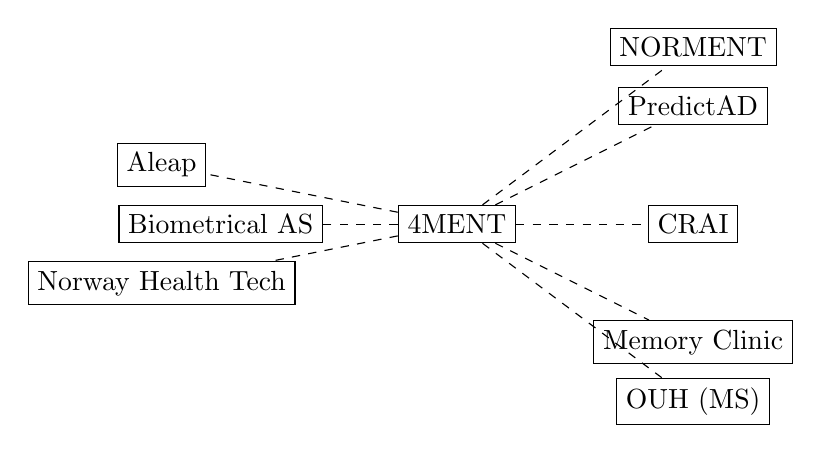
\begin{tikzpicture}
			\node[draw=black] (4ment) at (0, 0) {4MENT};
			\node[draw=black] (crai) at (3, 0) {CRAI};
			\node[draw=black] (norment) at (3, 2.25) {NORMENT};
			\node[draw=black] (predictad) at (3, 1.5) {PredictAD};
			\node[draw=black] (mc) at (3, -1.5) {Memory Clinic};
			\node[draw=black] (ms) at (3, -2.25) {OUH (MS)};
			\node[draw=black] (bio) at (-3, 0) {Biometrical AS};
			\node[draw=black] (nht) at (-3.75, -0.75) {Norway Health Tech};
			\node[draw=black] (aleap) at (-3.75, 0.75) {Aleap};

			\draw[dashed] (4ment) -- (bio);
			\draw[dashed] (4ment) -- (nht);
			\draw[dashed] (4ment) -- (aleap);

			\draw[dashed] (4ment) -- (norment);
			\draw[dashed] (4ment) -- (predictad);
			\draw[dashed] (4ment) -- (crai);
			\draw[dashed] (4ment) -- (mc);
			\draw[dashed] (4ment) -- (ms);
		\end{tikzpicture}
	\end{frame}

	\begin{frame}{Summary}
		\begin{itemize}
			\item There is a definite need and a rising interest for AI-based solutions in clinical health care
			\item We do research on technology with an emphasis on clinical use
			\item There are clinical environments eager to be part of operationalization in our immediate surrondings
			\item We are positioned in the center of excellent research environments, technology-enthusiastic clinicians, innovative decision makers, and aspiring technology clusters
		\end{itemize}
	\end{frame}
\end{document}
